\testCom
{%Номер задачи
	3.122
}
{%Условие
	условие
}
{%Дано
	дано
}
{%Найти
	найти
}
{%Решение
	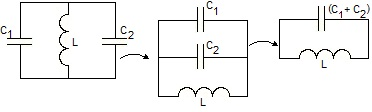
\includegraphics[height=30mm]{3_122.jpg}\\
	тогда:\\
	a) $ L \der{q}{t}{2} + \frac{q}{C_1 + C_2} = 0 \Rightarrow \omega^2 = \frac{1}{L(C_1 + C_2)} \quad T = 2 \pi \sqrt{(C_1 + C_2) L}$\\
	б) ЗСЭ:$ \frac{LI_A^2}{2} = \frac{(C_1 + C_2) U_A^2}{2}$ из условия $q(0) = U \dot q(0) = 0$\\
	$I_A = U \sqrt{\frac{C_1 + C_2}{L}}$\\
}

